%% General definitions
\documentclass{IEEEtran}
%\documentclass{article} %% Determines the general format.
\usepackage{a4wide} %% paper size: A4.
\usepackage[utf8]{inputenc} %% This file is written in UTF-8.
%% Some editors on Windows cannot save files in UTF-8.
%% If there is a problem with special characters not showing up
%% correctly, try switching "utf8" to "latin1" (ISO 8859-1).
\usepackage[T1]{fontenc} %% Format of hte resulting PDF file.
\usepackage{fancyhdr} %% Package to create a header on each page.
\usepackage{lastpage} %% Used for "Page X of Y" in the header.
                      %% For this to work, you have to call pdflatex twice.
\usepackage{enumerate} %% Used to change the style of enumerations (see below).
\usepackage{amssymb} %% Definitions for math symbols.
\usepackage{amsmath} %% Definitions for math symbols.
\usepackage{graphicx}
\usepackage{subfig}
\usepackage{wrapfig}
\usepackage{float}

\usepackage{tikz}
\usetikzlibrary{shapes,arrows}

%% Left side of header
\lhead{\course\\\semester\\Femur Segmentation Project}
%% Right side of header
\rhead{\authorname\\Page \thepage\ of \pageref{LastPage}}
%% Height of header
\usepackage[headheight=36pt]{geometry}
%% Page style that uses the header
\pagestyle{fancy}

% Define block styles
\tikzstyle{decision} = [diamond, draw, fill=blue!20, 
text width=5em, text badly centered, inner sep=0pt]
\tikzstyle{block} = [rectangle, draw, fill=blue!20, 
text width=5em, text centered, rounded corners, minimum height=4em]
\tikzstyle{line} = [draw, -latex']
\tikzstyle{cloud} = [draw, rectangle, rounded corners, fill=red!20,
minimum height=2em, text width=2.5cm, text badly centered]

\newcommand{\authorname}{Elias Arnold\\Alexander Luyten}
\newcommand{\semester}{Spring Semester 2019}
\newcommand{\course}{43075-01 Probabilistic Shape Modelling}
\author{Elias Arnold and Alexander Luyten}

\title{Project: Femur Segmentation}

\begin{document}
\maketitle
\begin{abstract}
The goal of this project is to segment femur bones in a CT scan, short for computed tomography. X-ray measurements, which are taken from different angles, produce a full three-dimensional image of the scanned body region.\par
To segment femur bones, we use a Statistical Shape Model (SSM) of the femur and modify it, such that it replicates the target bone in the CT scan as closely as possible. In addition to the Statistical Mesh Model, the Active Shape Model provides us with profiles, which are probability distributions of pixel intensities on lines perpendicular to the model surface.\par
The model fitting process is done using a Markov Chain Monte Carlo (MCMC) method called Metropolis-Hastings, which is a method for gaining samples from an unknown target distribution. In our case, the samples include the SSM coefficients, translation and rotation vector. Different samples are generated and evaluated using the profiles of the Active Shape Model, which gives us a likelihood that our current sample matches our CT scan.
\end{abstract}

\section{Methods}
	\begin{wrapfigure}{r}{0cm}
		\scalebox{.66}{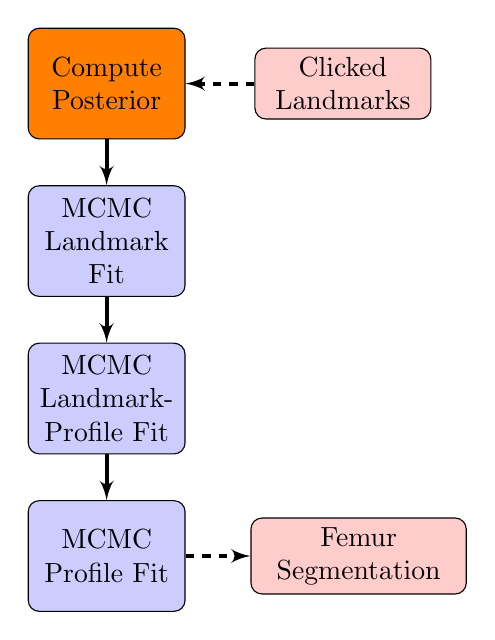
\begin{tikzpicture}[scale=0.2, node distance=2cm, auto]
	% Place nodes
	\node [block, fill=orange] (init) {Compute Posterior};
	%\node [cloud, left of=init, node distance=4cm] (lms) {clicked landmarks};
	\node [cloud, right of=init, text width=2cm, node distance=3cm, scale=1.0] (lms) {Clicked Landmarks};
	%\node [cloud, below of=lms] (rigid) {Rigid Alignment};
	\node [block, below of=init] (lmChain) {MCMC Landmark Fit};
	\node [block, below of=lmChain] (lmChainprofile) {MCMC Landmark-Profile Fit};
	\node [block, below of=lmChainprofile] (profileChain) {MCMC Profile Fit};
	\node [cloud, node distance=3.2cm, right of=profileChain] (lel) {Femur Segmentation};

	\path [line, line width=0.5mm] (init) -- (lmChain);
	\path [line, line width=0.5mm] (lmChain) -- (lmChainprofile);
	\path [line, line width=0.5mm] (lmChainprofile) -- (profileChain);
	%\path [line,dashed, line width=0.5mm] (rigid) -- (init);
	\path [line,dashed, line width=0.5mm] (lms) -- (init);
	\path [line,dashed, line width=0.5mm] (profileChain) -- (lel);
\end{tikzpicture}
}
		\caption{Femur segmentation pipeline}
		\label{fig:pipeline}
	\end{wrapfigure}
To obtain a femur segmentation, we perform a sequence of steps in our final pipeline, shown in Figure \ref{fig:pipeline}. First, we compute a posterior model using the clicked landmarks as observations. As determining the landmarks by clicking contains uncertainty, we added additional noise for the posterior at the landmarks. We then used the resulting posterior model as a starting point for the fitting process.\par
The fitting process consists of three different steps: Initially, we try to minimize the distances between the clicked landmarks and the corresponding points on the posterior model. After we have obtained a rough shape position estimation, we fit our model according to the given profiles and guide Metropolis-Hastings with the help of our landmarks. As a last refinement step, we approximate the fine shape deformations using only the profiles of the Active Shape Model and very small proposal steps. The resulting samples from each fitting step are the input of the next fitting step.

\subsection{Landmarks}
We manually clicked 20 landmarks in the given CT scan. To make this process not too time-consuming, we used the peaks of the bone shape (highest points of a structure, lowest points) as landmarks, which were relatively easy to find in the CT image, shown in Figure \ref{fig:1a}. Throughout the project, we assumed the clicked landmarks as ground truth observations and used them for different things like computing a posterior model, and as correspondent points for the MCMC fitting process.

\begin{figure*}[h]
	\subfloat[Landmark on the given bone model. Here, the highest point is choosen as a landmark.]{
		\begin{minipage}[c]{0.48\textwidth}
			\centering
			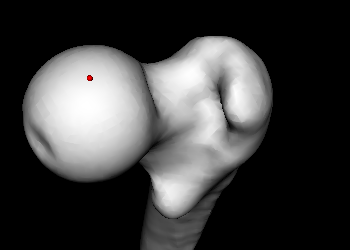
\includegraphics[width=1\textwidth]{img/topLandmarkPoint.png}
			\label{fig:1a}
	\end{minipage}}
	\hfill
	\subfloat[The original model (blue), and the resulting posterior (red)]{
		\begin{minipage}[c]{0.48\textwidth}
			\centering
			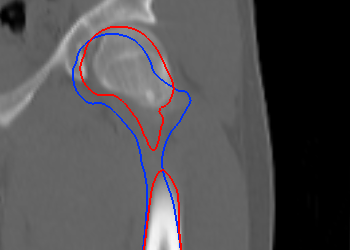
\includegraphics[width=1\textwidth]{img/topLandmarkPoint_posterior.png}
			\label{fig:1c}
	\end{minipage}}
	\caption{From the initial model to the posterior model using landmarks.}
\end{figure*}

\subsection{Posterior Model}\label{posterior}
After clicking the landmarks, we calculate a posterior model, which approaches all manually clicked landmarks.
A problem that occurred, was that some landmark points were not automatically in correspondence, because the orientation of the bone can differ. To compensate for this issue and errors from landmark selection, we used an uncertainty of 5mm for the posterior computation. This had the effect, that the posterior model did not necessarily have to hit all the landmark points exactly.

\subsection{Markov Chain Monte Carlo}
As previously mentioned, MCMC lets us draw samples from an unknown target distribution. In our case, a sample consists of our Statistical Mesh Model coefficients, a translation, and rotation vector. The method produces a Markov chain, where each sample only depends on the last sample, and converges to an equilibrium distribution, which is our target distribution.\par
The Metropolis-Hastings Algorithm is used to produce the Markov chain, which matches our target distribution in the limit. It works by taking a proposal distribution $Q(x'|x)$, which generates new samples according to the last sample, and a target distribution $P(x)$, which evaluates the likelihood of a sample. The algorithm is initialized with an arbitrary sample. To generate a new sample, we perform a random step starting from our old sample. The size and the direction of the step is drawn from $Q(x'|x)$. The new sample is accepted if it is more likely than our previous sample, but there is also a chance for less likely samples to get accepted. This allows the Markov chain to escape local minima.\par
In the following two subsections, we present two approaches to evaluate our samples and give insight on how proposals are generated. In our fitting process, the best sample of each Markov chain is the input of the next chain.

\subsubsection{Landmark Fitting}
As a starting point, we wanted to gain an accurate orientation of the bone in the CT scan. Because our posterior was not that accurate and we treated our landmarks as ground truth observations, we performed a landmark fit, which means that we wanted to find a sample, which matches our target landmarks the best. As Metropolis-Hastings generates samples from an entire distribution, but we are only interested in the best sample, we took the maximum a posteriori solution of all generated samples. In this step we allow the samples to change only the rotation and the position of the model, but the shape remains constant.

\subsubsection{Profile Fitting}
We also perform profile fitting, where we tried to approximate the shape of the target bone as closely as possible according to the gradients in the CT scans. We had 500 profiles given, that were perpendicular to the surface of the reference mesh. These profiles are essentially probability distributions which can be used to compute the likelihood of an image point to be part of the final target surface. To assess the likelihood of points, the method uses the intensity values of the image points. Here, mostly the shape is changed according to the profiles, but we also allow the model to rotate or translate at very small steps, so translation and rotation errors are not explained with shape deformations.

\subsubsection{Landmark-Profile Fitting}
To prevent the profile fitting method from making "bad" decisions, we weight the likelihood computation by the correspondence evaluator. We often had the error, that the profile evaluator changed the shape at critical areas, like the hip-joint area. There, the evaluator often pulled the shape outwards towards the hip-joint. To solve this problem, we use a guided profile evaluator, which is heavily weighted with the landmark evaluator. This enforces the profile exploration not too far away from the clicked landmarks.

\section{Results}
For the segmentation, we tried two different approaches. First, using the initial posterior model computation method mentioned in section \ref{posterior}. Second, we tried a simpler approach without initial computation, by simply performing the Metropolis-Hastings algorithm on the given femur model. As we were able to evaluate our different approaches on the given test data set with ground truth meshes, we were able to compare both approaches using the average mesh distances. The results are summarized in Table \ref{avgdistances} and indicate, that the simpler approach performs better. This can be seen in Figure \ref{comparison}. This may be due to the lower variability on the posterior model and the inability to explain the same range of bone shapes as the initial model.\par
The final segmentations of the target bones, without posterior model are visually accurate and close to the CT scan.

\begin{table}[h]
\centering
\begin{tabular}{l|c|c}
average distance & without posterior & with posterior\\
\hline
femur 4 & 0.55 & 0.99 \\
femur 14 & 0.51 & 1.53 \\
femur 23 & 0.71 & 1.63 \\
femur 25 & 0.53 & 1.16 \\
femur 30 & 0.58 & 1.21\\
\end{tabular}
\caption{Average distance results of both fitting approaches}
\label{avgdistances}
\end{table}

\newpage

\section{Conclusion}
The goal of the project was to perform a segmentation of a femur bone on a CT scan. We did this using Metropolis-Hastings with different proposals and evaluators. In addition to the Statistical Mesh Model of the femur bone, an Active Shape Model was also given, which includes pixel intensity distributions perpendicular to the model surface.\par
Our idea was to first compute a posterior model as an initialization step and then fit our posterior model using Metropolis-Hastings. The evaluation of the samples was based on the profiles of the Active Shape Model and the manually clicked landmarks.\par
To our surprise, the segmentations are better using the initial model without additional computation of the posterior model. We suspect that by calculating the posterior, our femur model loses a lot of its variance, so that it is no longer capable of explaining all possible femur shapes.\par
The results of our segmentation on the test data set, seen in Table \ref{avgdistances} indicate, that our fitting method produces good results, with an average of 0.576 mm average distance error per test bone. For the next time, the parameters for the proposals could be chosen more carefully, through systematic grid search, also samples could be saved over many runs, so that comparing old samples with new samples would be easier.

\begin{figure}[h]
	\centering
	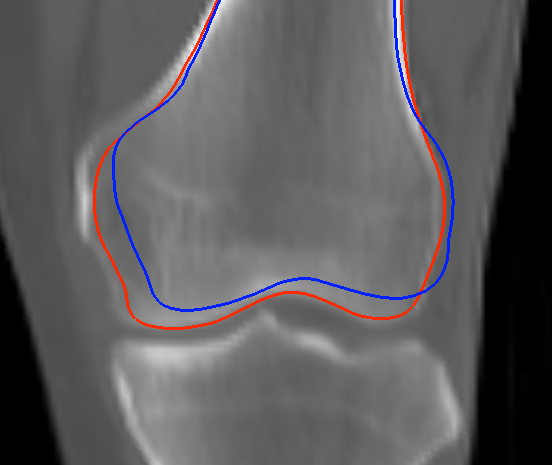
\includegraphics[width=.3\textwidth]{img/conclusion_image.png}
	\label{fig:conclusion_image}
	\caption{The same CT image segmented with an initial posterior computation (blue) and without (red). It can be seen that the version without an initial posterior computation actually fits the depicted bone better.}
	\label{comparison}
\end{figure}
\end{document}
